\documentclass[
  bibliography=totoc,     % Literatur im Inhaltsverzeichnis
  captions=tableheading,  % Tabellenüberschriften
  titlepage=firstiscover, % Titelseite ist Deckblatt
]{scrartcl}

% Paket float verbessern
\usepackage{scrhack}

% Warnung, falls nochmal kompiliert werden muss
\usepackage[aux]{rerunfilecheck}

% unverzichtbare Mathe-Befehle
\usepackage{amsmath}
% viele Mathe-Symbole
\usepackage{amssymb}
% Erweiterungen für amsmath
\usepackage{mathtools}

% Fonteinstellungen
\usepackage{fontspec}
% Latin Modern Fonts werden automatisch geladen
% Alternativ zum Beispiel:
%\setromanfont{Libertinus Serif}
%\setsansfont{Libertinus Sans}
%\setmonofont{Libertinus Mono}

% Wenn man andere Schriftarten gesetzt hat,
% sollte man das Seiten-Layout neu berechnen lassen
\recalctypearea{}

% deutsche Spracheinstellungen
\usepackage[ngerman]{babel}


\usepackage[
  math-style=ISO,    % ┐
  bold-style=ISO,    % │
  sans-style=italic, % │ ISO-Standard folgen
  nabla=upright,     % │
  partial=upright,   % ┘
  warnings-off={           % ┐
    mathtools-colon,       % │ unnötige Warnungen ausschalten
    mathtools-overbracket, % │
  },                       % ┘
]{unicode-math}

% traditionelle Fonts für Mathematik
\setmathfont{Latin Modern Math}
% Alternativ zum Beispiel:
%\setmathfont{Libertinus Math}

\setmathfont{XITS Math}[range={scr, bfscr}]
\setmathfont{XITS Math}[range={cal, bfcal}, StylisticSet=1]

% Zahlen und Einheiten
\usepackage[
  locale=DE,                   % deutsche Einstellungen
  separate-uncertainty=true,   % immer Unsicherheit mit \pm
  per-mode=symbol-or-fraction, % / in inline math, fraction in display math
]{siunitx}

% chemische Formeln
\usepackage[
  version=4,
  math-greek=default, % ┐ mit unicode-math zusammenarbeiten
  text-greek=default, % ┘
]{mhchem}

% richtige Anführungszeichen
\usepackage[autostyle]{csquotes}

% schöne Brüche im Text
\usepackage{xfrac}

% Standardplatzierung für Floats einstellen
\usepackage{float}
\floatplacement{figure}{htbp}
\floatplacement{table}{htbp}

% Floats innerhalb einer Section halten
\usepackage[
  section, % Floats innerhalb der Section halten
  below,   % unterhalb der Section aber auf der selben Seite ist ok
]{placeins}

% Seite drehen für breite Tabellen: landscape Umgebung
\usepackage{pdflscape}

% Captions schöner machen.
\usepackage[
  labelfont=bf,        % Tabelle x: Abbildung y: ist jetzt fett
  font=small,          % Schrift etwas kleiner als Dokument
  width=0.9\textwidth, % maximale Breite einer Caption schmaler
]{caption}
% subfigure, subtable, subref
\usepackage{subcaption}

% Grafiken können eingebunden werden
\usepackage{graphicx}

% schöne Tabellen
\usepackage{booktabs}

% Verbesserungen am Schriftbild
\usepackage{microtype}

% Literaturverzeichnis
\usepackage[
  backend=biber,
]{biblatex}
% Quellendatenbank
\addbibresource{lit.bib}
\addbibresource{programme.bib}

% Hyperlinks im Dokument
\usepackage[
  german,
  unicode,        % Unicode in PDF-Attributen erlauben
  pdfusetitle,    % Titel, Autoren und Datum als PDF-Attribute
  pdfcreator={},  % ┐ PDF-Attribute säubern
  pdfproducer={}, % ┘
]{hyperref}
% erweiterte Bookmarks im PDF
\usepackage{bookmark}

% Trennung von Wörtern mit Strichen
\usepackage[shortcuts]{extdash}

\author{%
  Toby Teasdale\\%
  \href{toby.teasdale@tu-dortmund.de}{toby.teasdale@tu-dortmund.de}%
  \and%
  Erich Wagner\\%
  \href{erich.wagner@tu-dortmund.de}{erich.wagner@tu-dortmund.de}%
}
\publishers{TU Dortmund – Fakultät Physik}


\subject{V203}
\title{Verdampfungswärme und Dampfdruckkurve}
\date{
  Durchführung: 14.12.2021
  \hspace{3em}
  Abgabe: 21.12.2021
}

\begin{document}

\maketitle
\thispagestyle{empty}
\tableofcontents
\newpage

\section{Ziel}
\label{sec:Ziel}

In dem Versuch \enquote{Brückenschaltung} werden unbekannte Wiederstände, Kapazitäten und Induktivitäten
gemessen. Dies geschieht durch diverse Brückenschaltungen. Außerdem wird die Frequenzabhänigigkeit der Brückenspannung
mithilfe einer sogenannten \textit{Wien-Robinson-Brücke} sowie der Klirrfaktor ermittelt.
\section{Theorie}
\label{sec:Theorie}

Zwei schwingende Systeme nennt man dann gekoppelt, wenn sie aufeinander eine Rückwirkung ausüben. 
Die Kopplung zweier schwingungsfähiger Systeme kann mithilfe äußerer Anregungen zur Energieübertragung gebracht werden, 
welche sich in Form von Resonanzeffekten erkennbar macht.\\
\\
Als ein gekoppeltes Schwingsystem sind zwei durch eine Feder verbundene Fadenpendel schwer zu untersuchen.
Es wird daher auf elektrische Schwingkreise zurückgegriffen, da Frequenz und Amplitude dabei leichter zu bestimmen sind.

\subsection {Verhalten kapazitiv gekoppelter Schwingkreise}

Es werden zwei identische Schwingkreise betrachtet, die durch eine Kapazität $C_\text{K}$ miteinander verbunden sind.

\begin{figure} 
    \centering
    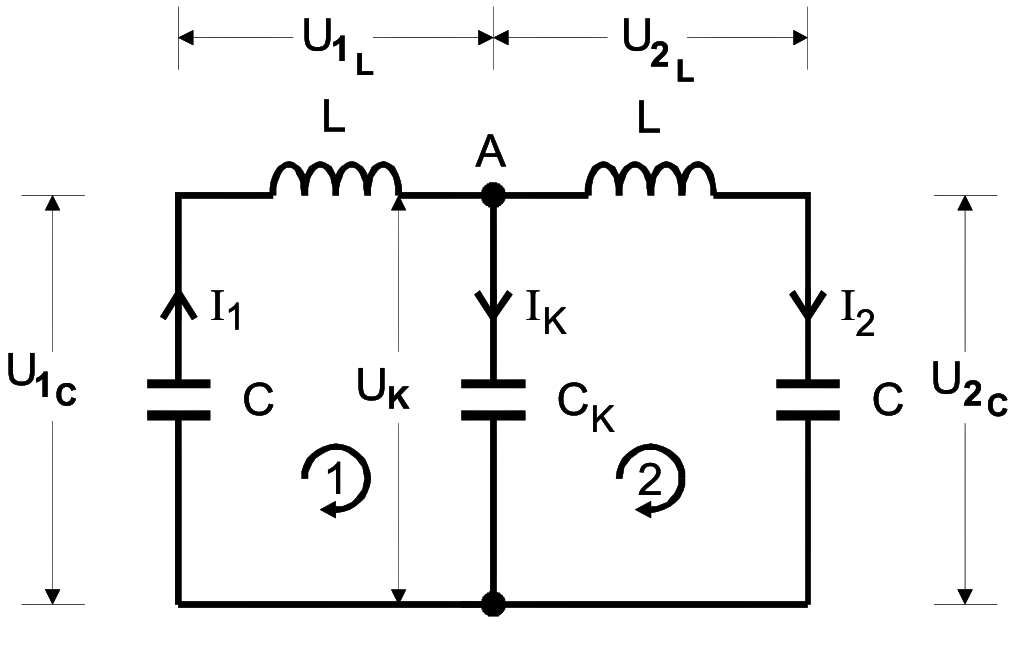
\includegraphics[width=10cm] {pictures/prinzipschaltbild.png}  
    \caption{Schaltung kapazitiv gekoppelter Schwingkreise. \cite{v355}}
    \label{fig:prinzipschaltbild}
\end{figure} 

Mithilfe der \textit{Kirchhoffschen Gesetze}, welche den Zusammenhang zwischen mehreren elektrischen Strömen und Spannungen 
beschreiben, ergibt sich im Knotenpunkt A
\begin{equation}
    I_{1} = I_\text{K} + I_{2} \,.
\end{equation}

Für Masche 1 und 2 ergibt sich
\begin{equation}
    U_{{1,2}_{C}} + U_{{1,2}_\text{L}} + U_\text{K} = 0 \,.
\end{equation}

In dieses Gleichungssystem werden die Beziehungen
\begin{equation} 
    U_{C} = \frac{1}{C} \dif{t} \int I \quad\text{und}\quad U_\text{L} = L \dot{I} \quad\text{ein.}
\end{equation}

eingesetzt. Damit ergeben sich für die beiden Maschen mit Differentiation nach $t$ die Differentialgleichungen
\begin{align}  
    L {\dot{I}}_{1} + \frac{1}{C} I_{1} + \frac{1}{C_\text{K}} (I_{1} - I_{2})  &= 0 \label{eq:dgl_1} \\
    L {\dot{I}}_{2} + \frac{1}{C} I_{2} + \frac{1}{C_\text{K}} (I_{1} - I_{2})  &= 0 \label{eq:dgl_2} \,.
\end{align}

Addition und Subtraktion der Gleichungen (\ref{eq:dgl_1}) und (\ref{eq:dgl_2}) ergibt die entkoppelten 
Differentialgleichungen für die neuen Variablen ($I_{1}+I_{2}$) und ($I_{1}-I_{2}$)
\begin{align} 
    L \frac {\dif{^2}} {\dif{t^2}} (I_{1} + I_{2}) + \frac{1}{C} (I_{1} + I_{2})  &= 0 \label{eq:dgl_1_entk} \\
    L \frac {\dif{^2}} {\dif{t^2}} (I_{1} - I_{2}) + \left( \frac{1}{C} + \frac{2}{C_\text{K}} \right) (I_{1} - I_{2})  &= 0 \label{eq:dgl_2_entk} \,.
\end{align}

Diese werden durch
\begin{align}
    (I_{1} + I_{2})(t) &= (I_{1,0} + I_{2,0}) \cos(I_{1} + I_{2}) \label{eq:dgl_1_sumsol} \\
    (I_{1} - I_{2})(t) &= (I_{1,0} - I_{2,0}) \cos \left( \frac {t} {{\sqrt [] {L \left( \frac{1}{C} + \frac{2}{C_\text{K}} \right)^{-1} }}} \right) \label{eq:dgl_2_sumsol}
\end{align}

gelöst. Durch erneute Addition und Subtraktion von (\ref{eq:dgl_1_sumsol}) und (\ref{eq:dgl_2_sumsol}) ergeben sich die Lösungen 
der ursprünglichen Ströme $I_{1}$ und $I_{2}$
\begin{align}
    I_{1}(t) &= \frac{1}{2} (I_{1,0} + I_{2,0}) \cos(2 \pi \nu^+ t)  +  \frac{1}{2} (I_{1,0} - I_{2,0}) \cos(2 \pi \nu^- t) \label{eq:dgl_1_sol} \\
    I_{2}(t) &= \frac{1}{2} (I_{1,0} + I_{2,0}) \cos(2 \pi \nu^+ t)  -  \frac{1}{2} (I_{1,0} - I_{2,0}) \cos(2 \pi \nu^- t) \label{eq:dgl_2_sol} \,,
\end{align}

wobei 
\begin{align}
    \nu^+ &= \frac {1} {2 \pi \sqrt[]{LC}} & \mbox{\centering und} && \nu^- = \frac {t} {2 \pi \sqrt [] {L \left( \frac{1}{C} + \frac{2}{C_\text{K}} \right)^{-1} }}
\end{align}

die Schwingungsfrequenzen von (\ref{eq:dgl_1_sumsol}) und (\ref{eq:dgl_2_sumsol}) darstellen. \\
\\
Sind zu Beginn die Amplituden beider Schwingkreise gleich groß ($I_{1,0} = I_{2,0}$), so entfallen bei (\ref{eq:dgl_1_sol}) und (\ref{eq:dgl_2_sol})
die jeweils letzten Terme. In diesem Fall schwingen die beiden Schwingkreise gleichphasig mit der Schwingunsfrequenz $\nu^+$, am
Koppelkondensator $C_\text{K}$ leigt dabei nie eine Spannung an. Bei gegengleichen Amplituden ($I_{1,0} = -I_{2,0}$) schwingen die Schwingkreise gegenphasig
mit der erhöhten Schwingunsfrequenz $\nu^-$ und die Spannung an $C_\text{K}$ wird maximal. Diese beiden Schwingungstypen werden \textit{Fundamentalschwingungen} genannt. \\
\\
Wird hingegen nur einer der beiden Schwingkreise ausgelenkt ($I_{1,0} \neq 0, I_{2,0} = 0$), so ergeben sich Schwebungen.
\begin{align}
    I_{1}(t) &= I_{1,0} \cos(\pi (\nu^+ + \nu^-) t) \cos(\pi (\nu^+ - \nu^-) t) \label{eq:dgl_1_sol_schweb} \\
    I_{2}(t) &= I_{1,0} \sin(\pi (\nu^+ + \nu^-) t) \sin(\pi (\nu^+ - \nu^-) t) \label{eq:dgl_2_sol_schweb} 
\end{align}

Der Verlauf der Ströme $I_{1}(t)$ und $I_{2}(t)$ werden in Abbildung (\ref{fig:schwebung}) dargestellt.
\begin{figure} 
    \centering
    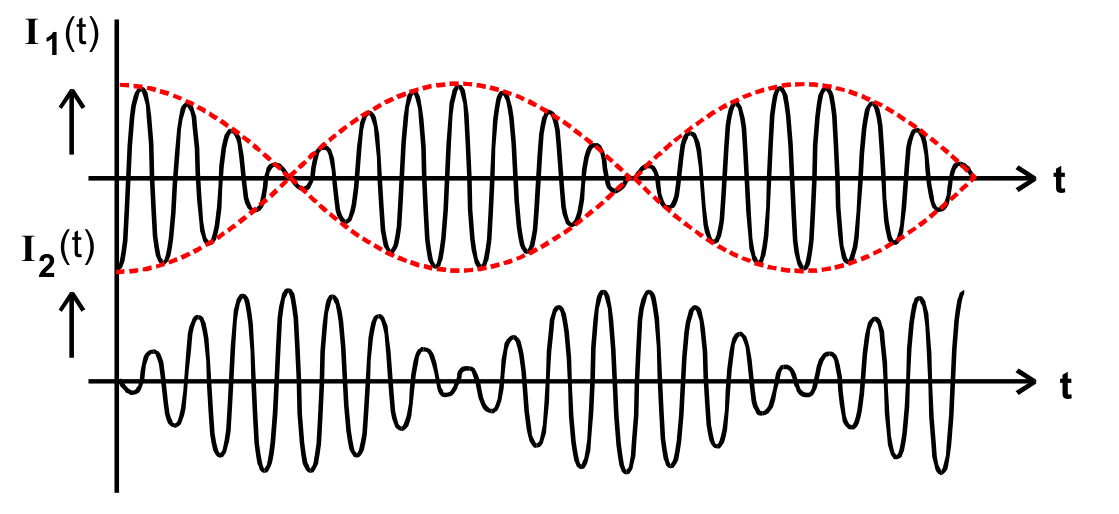
\includegraphics[width=10cm] {pictures/schwebung.png} 
    \caption{Zeitlicher Verlauf der Ströme im Falle einer Schwebung. \cite{v355}}
    \label{fig:schwebung}
\end{figure} 

Bei diesen Anfangsbedingungen wird die Energie des ausgelenkten Schwingkreises auf den ruhenden übertragen, was eine gekoppelte Schwingung zur Folge hat.
Die Amplitude der Schwingungsfrequenz ändert sich mit der \textit{Schwebungungsfrequenz} 
\begin{align}
    \nu_\text{Schwebung} &= \nu^- - \nu^+ \., \\
    \intertext{während das System mit der Schwingungsfrequenz}
    \nu_\text{Schwingung} &= \frac{1}{2} \left( \nu^+ + \nu^- \right) \approx \nu^+ 
\end{align}
schwingt.


\subsection {Abhängigkeit des Stromes von der Frequenz}

Werden die Schwingkreise durch eine von außen angelegte Sinusspannung angeregt (siehe Abblildung \ref{fig:sinusspannung}), \\
\begin{figure} 
    \centering
    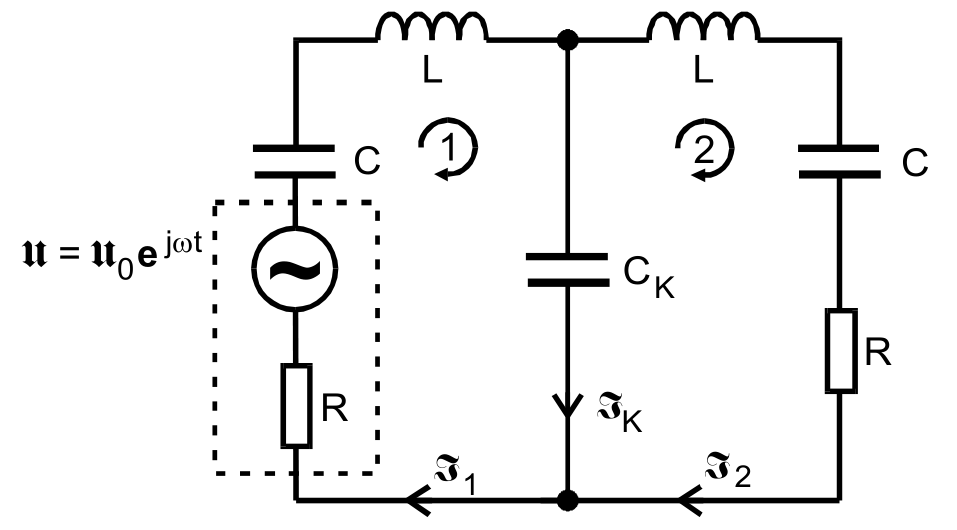
\includegraphics[width=10cm] {pictures/sinusspannung.png} 
    \caption{Schwingkreise mit Sinusgenerator. \cite{v355}}
    \label{fig:sinusspannung}
\end{figure} 

so ergeben sich mithilfe der \textit{Kirchhoffschen Maschenregel} die Gleichungen
\begin{align}
    U &= (z_{C} + z_\text{L} + z_{C_\text{K}} + z_{R}) I_{1} - z_{C_\text{K}} I_{2} \label{eq:sin_masche_1} \\
    0 &= (z_{C} + z_\text{L} + z_{C_\text{K}} + z_{R}) I_{2} - z_{C_\text{K}} I_{1} \label{eq:sin_masche_2} 
\end{align}

mit den Impedanzen
\begin{align} 
    z_{C} &= \frac{1}{i \omega C} & z_\text{L} = i \omega L  && z_{R} = R \,.
\end{align}

Nach Elimination von $I_{1}$ folgt für $I_{2}$ 
\begin{align}
    I_{2} &=U \frac{\frac{1}{i \omega C_\text{K}}}{\left(i \omega L+\frac{1}{i \omega C}+\frac{1}{i \omega C_\text{K}}+R\right)^{2}+\frac{1}{\omega^{2} C_\text{K}^{2}}} \label{eq:strom2} \\
    \Rightarrow\left|I_{2}\right| &=\lvert U\rvert \frac{1}{\sqrt{4 \omega^{2} C_\text{K}^{2} R^{2} Z(\omega)^{2}+\left(\frac{1}{\omega C_\text{K}}-\omega C_\text{K} Z(\omega)^{2}+\omega R^{2} C_\text{K}\right)^{2}}} \label{eq:betrag_strom2}     
\end{align}

mit
\begin{align}
    Z(\omega)=\omega L-\frac{1}{\omega\left(\frac{1}{C}+\frac{1}{C_\text{K}}\right)^{-1}} \,.
\end{align}

Der Strom $I_{2}$ nimmt für $\nu^+$ und $\nu^-$ seine Maxima an:
\begin{align}
    \left|I_{2}\left(\omega^{+}\right)\right| &= \frac{1}{R \sqrt{4+\frac{R^{2} C_\text{K}^{2}}{L C}}} \label{eq:strom2_omegaplus}\\
    \left|I_{2}\left(\omega^{-}\right)\right| &= \frac{1}{R \sqrt{4+\frac{R^{2} C_\text{K}^{2}}{L C}\left(1+\frac{C}{C_\text{K}}\right)}} \label{eq:strom2_omegaminus}
\end{align}

\section{Durchführung}
\label{sec:Durchführung}

\subsection{Bestimmung der Zeitkonstanten}
\begin{figure}
    \centering
    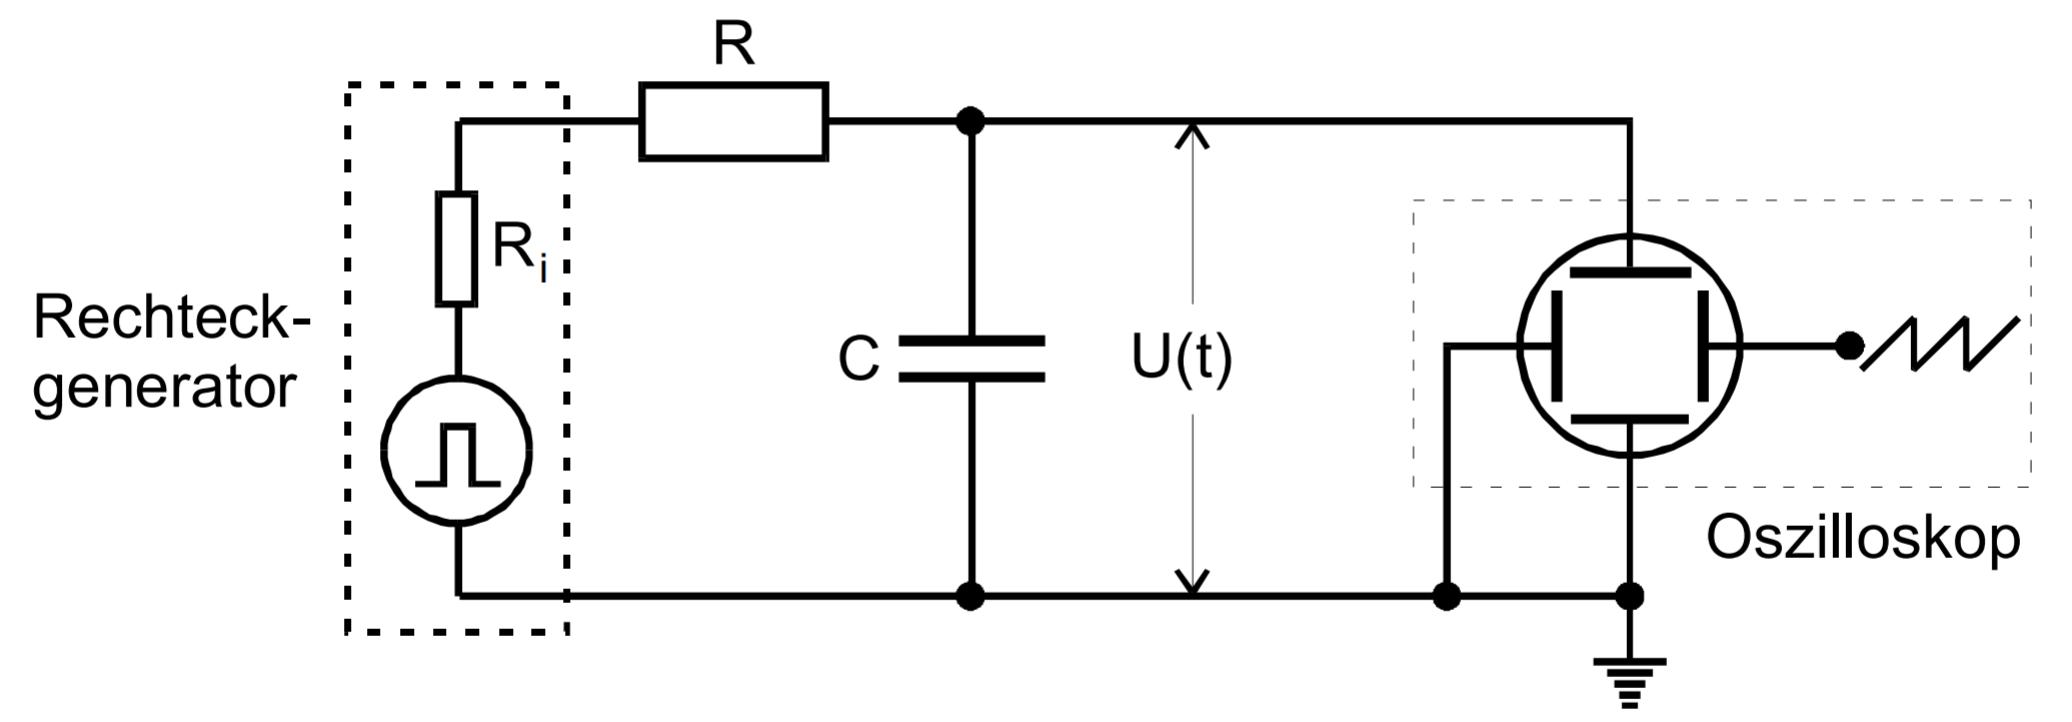
\includegraphics[width=\textwidth]{pictures/zeitkonstante.png}
    \caption{Schaltung zur Messung der Zeitkonstanten \cite{v353}.}
    \label{fig:zeitkonstante}
\end{figure}

Um die Zeitkonstante zu bestimmen, wird zunächst der RC-Kreis wie in Abbildung \ref{fig:zeitkonstante}
an ein Oszilloskop angeschlossen und mit einem Rechteckpuls $U_0 (t)$ angeregt.
Dabei ist der Widerstand $R$ und die Kapazität $C$ unbekannt.
Dann wird mit Hilfe des Triggers die Entladekurve der Kondensatorspannung $U_C (t)$ fixiert und
zu verschiedenen Zeiten $t$ notiert.

\subsection{Messung der Frequenzabhängigkeit und Phasenverschiebung}

\begin{figure}
    \centering
    \includegraphics[width=\textwidth]{pictures/Phasenverschiebung.png}
    \caption{Skizze einer Phasenverschiebung zweier Spannungen \cite{v353}.}
    \label{fig:zeitkonstante}
\end{figure}

Nun soll die Frequenzabhängigkeit der Kondensatorspannung $U_C$ und die jeweilige
Phasenverschiebung zur Generatorspannung bestimmt werden.
Dafür wird die Anregungsfrequenz auf eine Sinusanregung umgestellt.
Es werden also jeweils die Frequenz $f$, die Phasenverschiebung $\phi$ und die Spannung $U_C$ notiert.
Die Phasenverschiebung wird am Oszilloskop einfach abgelesen, indem das Oszilloskop so eingestellt wird,
dass die beiden Symmetriepunkte der Generatorspannung und der Kondensatorspannung im Mittelpunkt sind.
Die Amplitude der Kondensatorspannung kann dann auch einfach abgelesen werden.
Die Frequenz wird einfach am Gerät eingestellt und notiert.

\subsection{Dreiecksanregung eines RC-Kreises}

Am Schluss soll noch der RC-Kreis aus Abbildung \ref{fig:zeitkonstante} mit einer Dreiecksanregung angeregt werden
und dann für hohe Frequenzen beobachtet werden.
Dafür wird am Generator auf Dreiecksanregung gestellt und eine Frequenz von $f \geq 10 \si{\kilo\hertz}$ gewählt.
\section{Fehlerrechnung}
\label{sec:Fehlerrechnung}

Im Folgenden wird die allgemeine Fehlerrechnung und alle wichtigen Größen der entsprechenden Rechnung erklärt.
Die wichtigsten Werte dabei sind der 
\begin{align}
    \text{Mittelwert} \quad & \bar{x}  = \frac{1}{N} \sum_{i=0}^{n} x_i \quad \text{und die} \label{eq:mittelwert} \\
    \text{Standartabweichung} \quad & \sigma  = \sqrt{\frac{1}{N - 1 } \sum_{i=0}^{N} (x_i -  \bar{x})^2} \, . \label{eq:standartabweichung}
\end{align}
Dabei entspricht $x_i$ einer $N$-fach gemessenen Größe, die jeweils mit einem Fehler versehen ist.

Entstehen mehrere Unbekannte in einer Messung, folgen daraus auch mehrere Messunischerheiten,
die in dem weiteren Verlauf der Rechnung berücksichtigt werden müssen.
Es gilt die \textit{Gaußsche Fehlerfortplanzung}
\begin{equation}
    \increment f(y_1 ,y_2 ,...,y_N ) = \sqrt{\left(\frac{\dif{f}}{\dif{y_{1}}} \increment y_{1}\right)^2
    + \left(\frac{\dif{f}}{\dif{y_{2}}} \increment y_{2}\right)^2 + ... + 
    \left(\frac{\dif{f}}{\dif{y_{N}}} \increment y_{N}\right)^2
    } \, . \label{eq:fehlerfortplanzung}
\end{equation}
\section{Auswertung}
\label{sec:Auswertung}

\subsection{sec:LangeSpuleAuswertung}

Im folgenden wird die magnetische Flußdichte einer langen Spule gemessen und graphisch dargestellt.

\section{Diskussion}
\label{sec:Diskussion}

Auffällig ist, dass die Werte der Zeitkonstanten nah bei einander liegen und generell die
experimentellen Graphen meist den theoretischen, erwarteten Graphen sehr ähnlich sind.
Die Entladekurve des Kondensators entspricht einem erwarteten exponentiellen Abfall der
Spannung. Die Amplitude der Kondensatorspannung sinkt mit zunehmender Frequenz
ebenfalls wie erwartet exponentiell. Auch die Phasenverschiebung bleibt wie erwartet
zwischen 0 und $\pi/2$. Die Zeitkonstante kann über die drei Messreihen ausgerechnet
werden. Der genauen Wert für der Zeitkonstante kann nicht weiter berechnet werden, da
der Ohmsche Widerstand R des Widerstand und die Kapazität C des Kondensators nicht
gegeben sind und keine Messgeräte vorhanden sind. Die gemessene Zeitkonstante über
die Methode der Entladung des Kondensators ist 2.03 mal kleiner als die Zeitkonstante
aus der Messreihe zur Methode der Amplitude in Abhängigkeit von der Freqenz. Die
Zeitkonstante aus der Messung der Amplitude in Abhängigkeit von der Freqenz ist
2.69 mal kleiner als der Wert aus der Methode über die Phasenverschiebung zwischen
Generator- und Kondensatorspan- nung. Diese Abweichungen können unter anderem
daher kommen, dass eine geringer Ablesefehler auf dem Oszilloskop nicht ausgeschlossen
werden kann.

\newpage
\printbibliography{}
\nocite{matplotlib}
\nocite{numpy}
\nocite{scipy}
\nocite{uncertainties}
\nocite{reback2020pandas}

\end{document}
